\chapter{Package improvements implementation}
\label{ch:implementation}

\section{Administration requirements}
One of the administrator's main tasks while managing networks is, if required, to facilitate the coexistence of different Routing protocols in the same network section. Hence the requirement of rich routing tools as Quagga or Bird to act as facilitators of this route \textit{crossed-announcement} -and even attributes translation- between protocols.

Administrators require:
\begin{itemize}
    \item A full-featured tool with an easy and intuitive UI to manage and monitor protocol health and data efficiently and avoiding any handmade/custom edit, reducing configuration's complexity.
    \item Use of LEDE/OpenWRT-based firmwares widely used in the target network.
    \item A Routing protocols management tool that, at least, supports BGP Static Routing Protocol and it is able to share routes with BMX6 Dynamic Routing Protocol in a manageable way.
    \item Use Bird Daemon instead of Quagga to make us of its proven efficiency, low resource consumption and powerful filter capabilities, which is critical to some of the widely used commodity hardware in Guifi.net.
    \item Use and improve Bird Daemon's configuration integration package (bird-uci and luci-app-bird) available in the official Routing Repository of LEDE/OpenWRT.
    \item Avoid project-specific customisations in the integration package that would not benefit all the community. If required, add those custom enhancements in a development branch.
    \item Update Package's documentation and create new topics to cover Web UI interface and any manual process not covered by package's improvements.
    \item Update Bird integration package in order to be compliant to the latest API (v1.6.3 when this document was written).
    \item Enhance Web UI to support user-friendly configuration and visualisation of the following:
    \begin{itemize}
        \item Bird Daemon service status
        \item Bird Daemon events information (Logs)
        \item Filters and Functions editing using an embedded HTML text editor.
        \item Update old configuration Web pages, fix some outdated options and re-sort them to a more logically order.
    \end{itemize}
    \item Do theoretical viability investigation to use uBus Daemon as a mechanism to communicate with Bird Daemon and get health information and current-status information for handled protocol using JSON messages.
\end{itemize}

\section{Changes and improvements implemented}
The following sections summarises what has been changed as part of this project's development, which changes have been successful, challenges found and lessons learnt that will help towards future versions of the Package.

\subsection{Build and deployment process documentation update}
One of the first challenges I found during the initial investigation was that the documented process for building the package was wrong. This misalignment led into few days testing the build process using the latest version of the development environment in order to tune it (the original building process was documented in 2014).

\begin{itemize}
    \item Generalise Makefiles (bird4/bird6) and post installation scripts.
    \item Add detailed steps to get Package's source, add bird required packages into the Image Build settings, compile it (\texttt{make}) and deploy it in the target router.
    \item Add alternative mechanisms, Package information and (after finishing changes in the Package), Package known issues.
\end{itemize}

\subsection{Apply code standards}
As a daily Bash user, one of the main concerns that I had once I did retake the project was the state of the code because I did stop giving support to the Package on 2014 and I have improved drastically my consciousness towards clean, standard and following-best-practises code. Therefore, the top priority task I got was to normalise the code, apply best practises and, where possible, refactor it to follow a \textit{library}-pattern to be able to formalise an API and, in future releases, even to create unitary tests that would automate Package's tests.

The first challenge I found was that LEDE/OpenWRT firmwares use the light compound of Linux tools BusyBox\footnote{\href{https://busybox.net/downloads/BusyBox.html}{BusyBox}: light and optimised UNIX tools including most of the widely used terminal commands (i.e. \texttt{ash}, \texttt{cat} or \texttt{rm}).}. This all-in-one tool comes really handy in embedded environments where performance and storage are critical but some of its tools are limited versions of the original ones.

Particularly, the tool that has been more challenging is \textit{ash}, which is the built-in Shell Command Line included instead of \textit{Bash} and, although it includes most of its features, there are few others like Arrays that are not available and requires the developer to re-think the solution (Ash readme page suggest the use of \texttt{set} command).

Some examples of the improvements applied are:
\begin{itemize}
    \item Encapsulate variables with curly brackets to avoid wrong substitutions or other common issues where mixing variable names and other strings:
    \begin{lstlisting}[language=bash,caption={Variable encapsulation}]
root@LEDE:~# path="/etc/"
root@LEDE:~# ls $pathconfig/bird4
ls: /bird4: No such file or directory
root@LEDE:~# ls ${path}config/bird4
/etc/config/bird4
\end{lstlisting} 
    This is a forced example but there are some instances where, in really complex scripts, unexpected substitutions could happen.
    \item Encapsulate Strings appropriately to avoid unexpected substitutions or code execution (i.e. script injection): this is an uncommon situation that could happen with commands like \texttt{sed}, where quotes and other special symbols are crucial to get the expected output.
    \item Use of 4 spaces instead of tabs for code readability.
    \item Use of simplified \texttt{if} statements \textbf{only} with clear and single-line occasions. Avoid using simplifications on instances where more than one line is required or the command is too large and would be more reasonable to split it using backslash (\texttt{\textbackslash}).
    
Acceptable:
\begin{lstlisting}[language=bash,caption={If statement simplification (I)}]
root@LEDE:# var="true"
root@LEDE:# [ "$var" = "true" ] && install_package="y" || install_package="n"
var is true
\end{lstlisting}
Unacceptable:
\begin{lstlisting}[language=bash,caption={If statement simplification (II)}]
root@LEDE:# [ "$(uname)" = "Linux" ] && { . /etc/os-release;
 echo -e "\n $LEDE_RELEASE \n"; } || echo "Not Available"

LEDE Reboot SNAPSHOT r3969-8322dba

root@LEDE:#
\end{lstlisting}
\end{itemize}

\subsection{init.d script and service management}
\label{sec:initd}
Bird's init.d script (\texttt{/etc/init.d/bird4}) manages the service on boot or on demand. Bird Daemon's init.d file is substituted on installation time by \texttt{/etc/bird\{4|6\}/init.d/bird\{4|6\}} script, and the original one backed up as \texttt{/etc/bird\{4|6\}/init.d/bird\{4|6\}.orig} to be restorable in the event of uninstalling the Package.

Improvements introduced are:
\begin{itemize}
    \item Refactor init.d script and split it in two files. \texttt{bird\{4|6\}} for service management and \texttt{bird\{4|6\}-lib.sh} as an \textit{API/function} holder for UCI-bird configuration translation.
    \item Store a backup of the current configuration each time the service is started. However, this backup is overwritten each time and it is administrator decision to take a copy of this file before reloading the service.
    \item Add \textit{smart} service management to avoid multiple start/stop/restart calls to the service, causing service disruptions if not required (i.e. multiple start calls should be ignored). See figure \ref{fig:initdt}.
    \item Add extra management functions for LUCI Web management. These new functions call the original ones but forcing plain text outputs. See figure \ref{fig:initdui}.
    \item Re-sort UCI translation script's in order to fix an issue with Functions and Filters.
    \item Enhance service handling and error information logging, previously dismissed.
\end{itemize}

\begin{figure}[ht!]
    \centering
    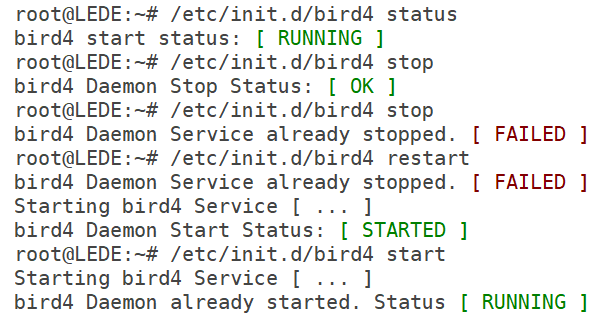
\includegraphics[width=0.7\textwidth]{images/initdterminal}
    \caption{Service management for Terminal.}
    \label{fig:initdt}
\end{figure}

\begin{figure}[ht!]
    \centering
    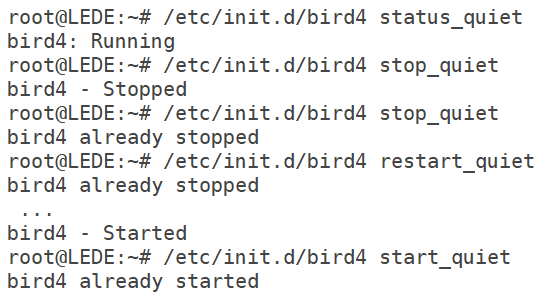
\includegraphics[width=0.7\textwidth]{images/initdui}
    \caption{Service management for Web UI.}
    \label{fig:initdui}
\end{figure}

\subsection{UCI Configuration improvements}
\label{sec:uciimp}
The Unified Configuration Interface (UCI) aims to centralise OpenWrt's settings and it is widely used for almost, if not all, the packages in OpenWrt. UCI allows you to easily, and in a human-readable manner, configure any system following the same scheme, simplifying administration overheads.

However, \textit{bird-uci} Package uses the UCI configuration file in a non-classical manner. Instead of making use of the configuration as it is, the Package only acts as a translator between what the user wants (written in UCI-scheme) and what bird needs to work (c-like configuration file). As stated in section \ref{sec:motivation}, the first version of the package successfully manages Bird, but there have been some API changes since Bird v1.4.3 and the integration is not completed yet:

\begin{itemize}
    \item As part of Bird's v1.4.3 to v1.6.3 API reviewing, some options have required tweaking in order to be compliant to the latest API.
    \item Most of the UCI improvements are tied to LUCI improvements (see section \ref{sec:luciimp}) in order to enhance User eXperience.
    For example, BGP Protocol allows you to execute an action once a number of routes is reached (imported, exported or received). This is shown as a pair of settings in the UI. Previously, each setting was independent, which was a problem as both are optional and hidden for simplicity reasons.
    By adding the extra option, I have been able to tie both options graphically and make them work as expected.
    From /etc/config/bird4:
    \begin{lstlisting}[language=bash,caption={Tied options using UCI (I)}]
config bgp 'bgpAS1'
        option import_trigger '0'
        option export_trigger '0'
        option receive_trigger '0'
        option disabled '0'
        option template 'test123'
        option neighbor_address '192.168.1.100'
        option neighbor_as '1'
\end{lstlisting}

    As shown in the snippet, we have three \texttt{\_trigger '0'} options that states that there is \textbf{no} Limit set in this BGP session. However, if we set one through the UI:
    
\begin{figure}[H]
    \centering
    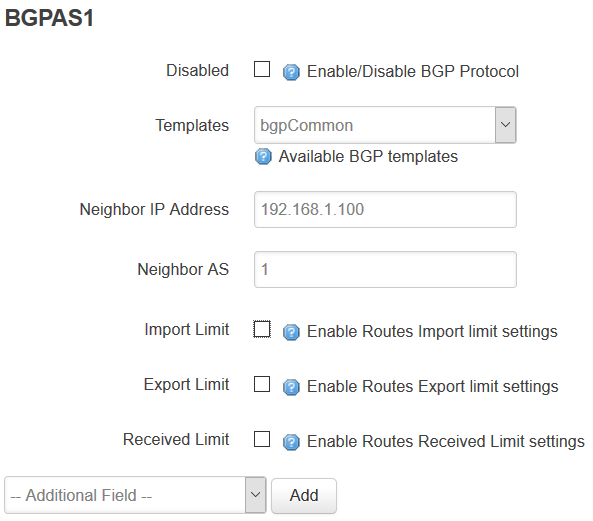
\includegraphics[width=0.8\textwidth]{images/bgp/bgptrigger1}
    \caption{Import Limit Trigger \textbf{not} selected.}
    \label{fig:uitiedn}
\end{figure}

\begin{figure}[H]
    \centering
    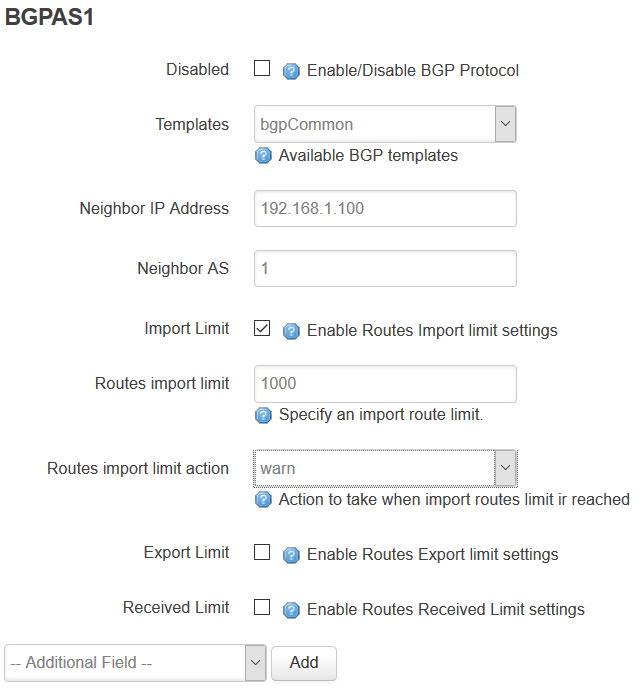
\includegraphics[width=0.8\textwidth]{images/bgp/bgptrigger2}
    \caption{Import Limit Trigger \textbf{selected}.}
    \label{fig:uitiedy}
\end{figure}

As shown in both figures \ref{fig:uitiedn} and \ref{fig:uitiedy} LUCI brings both options together, making it clear to the administrator that these settings must be filled. The UCI result for \ref{fig:uitiedy} is the following:

\begin{lstlisting}[language=bash,caption={Tied options using UCI (II)}]
config bgp 'bgpAS1'
        option import_limit_action 'warn'
        option export_trigger '0'
        option receive_trigger '0'
        option disabled '0'
        option template 'bgpCommon'
        option neighbor_address '192.168.1.100'
        option neighbor_as '1'
        option import_trigger '1'
        option import_limit '1000'
\end{lstlisting}

This \textit{tying} improvement has been done in the web UI's and not in UCI translation time because, as can be seen in the following code snippet, it is easier to let LUCI configuration management process to add/remove those attributes automatically on settings save time, than doing some hand-made if statements.

In the following LUA snippet, LUCI creates a UI Flag option (our trigger) which is mandatory (\texttt{optional = false}. The other two options (\texttt{limit} and \texttt{limit\_action}) are both optional and dependant on the value of our flag (\texttt{depends({import\_trigger = "1"})}.

\begin{lstlisting}[language=lua, caption={LUCI tied options implementation.}]
[...]
import_trigger = sect_templates:option(Flag, "import_trigger", "Import       Limit", "Enable Routes Import limit settings")
import_trigger.default = 0
import_trigger.rmempty = false
import_trigger.optional = false

import_limit = sect_templates:option(Value, "import_limit", "Routes import   limit", "Specify an import route limit.")
import_limit:depends({import_trigger = "1"})
import_limit.rmempty = true

import_limit_action = sect_templates:option(ListValue,                       "import_limit_action", "Routes import limit action", "Action to take when    import routes limit ir reached")
import_limit_action:depends({import_trigger = "1"})
import_limit_action:value("warn")
import_limit_action:value("block")
import_limit_action:value("disable")
import_limit_action:value("restart")
import_limit_action.default = "warn"
import_limit_action.rmempty = true
[...]
\end{lstlisting}
\end{itemize}

\newpage

\subsection{LUCI UI improvements}
\label{sec:luciimp}
Following previous section's UCI/LUCI example\ref{sec:uciimp}, there have been other UI improvements coupled with changes in the UCI implementation. The following subsections will cover each UI Page to summarise its role and which changes have been done to it. Nevertheless, the last subsection will explain the number of challenges faced during project's development. More detailed images of each page are located in the Appendix \ref{app:ch:extrap}. The ones shown here are for reference.

\subsubsection{Status Page}
\textbf{New} Page allowing an administrator to manage Bird Service. This page shows 3 buttons tied with the init.d functions explained in section \ref{sec:initd} figure \ref{fig:initdui}.


The contents of this page are:
\begin{itemize}
    \item Three buttons to trigger the service management: Start, Stop and Restart in Quiet mode.
    \item Dynamic Text Box showing Bird service's status. This text will be updated if you trigger any service update through the buttons.
\end{itemize}

\begin{figure}[H]
    \centering
    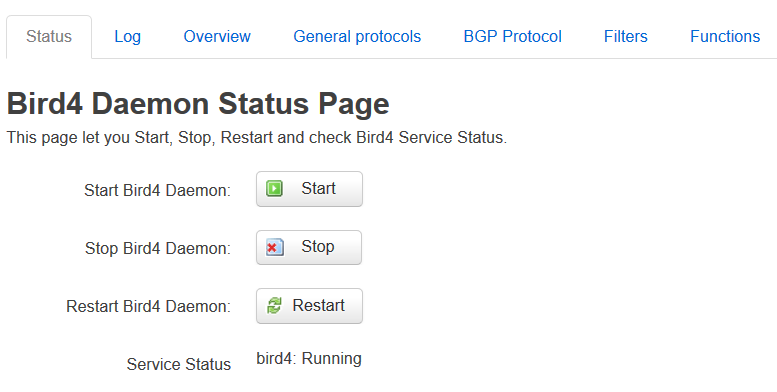
\includegraphics[width=0.8\textwidth]{images/bird0.3/status}
    \caption{Status Page}
    \label{fig:statusp}
\end{figure}

Although contents of this page are simple and straightforward, the result shown in figure \ref{fig:statusp} is not the desired one. The initial idea was to use a single button for starting and stopping the service, and none for restart. Moreover, the button would be automatically switch between states showing, when started, service's PID. In Appendix \ref{app:ch:extrap} you can see the expected behaviour shown in the LUCI implementation of Privoxy's OpenWrt Package.

The reason behind not doing it is that this simple change would require to change from using LUCI's CBI (Lua) to LUCI2 (JavaScript). Lua's implementation allows you to trigger a number of actions according to a specific element state, if an action (i.e. button clicked) is triggered or during page's rendering. However, there is no granular control on it or a polling mechanism that could automate the transition between service disabled and enabled. To do so, it would be required to force the page to wait (manual OS \texttt{sleep} command) which would also \textbf{block} page's loading.

Moreover, I did do a test implementation (without a \texttt{sleep}) and, because of the way CBIs work, the button action and rendering action were somehow triggering service calls multiple times, starting and stopping the service in an unexpected way and not refreshing the contents (wrong status and PID displayed).

\subsubsection{Log Page}
\textbf{New} Page showing contents in Bird's configured Log file. This page is automatically refreshed \textbf{each second} with the following information:

\begin{itemize}
    \item Name of the Log file. For reference and easier administration.
    \item Size of the Log file. Critical information in Bird configurations where \textbf{Debug} information is also enabled. Log file can grow really fast if there are more peers sharing information or if the debug mode is set to log most/all the possible events in the system.
    If the Log file grows enough to fill the /var partition, Bird will \textbf{automatically} shutdown and \textbf{prevent} any start up attempt until this is resolved. 
\end{itemize}

\begin{figure}[H]
    \centering
    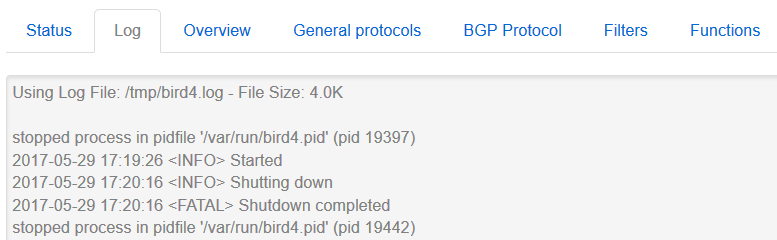
\includegraphics[width=\textwidth]{images/bird0.3/log}
    \caption{Log Page: service restart example}
    \label{fig:statusp}
\end{figure}

This page has been implemented using mixed capabilities from LUCI and LUCI2. Because of the requirement to show a \textbf{rolling} Log page with a reasonably regular auto-refresh process, it was necessary to use JavaScript's XHR capabilities embedded in the HTML page itself together with Lua code to read the file and send the text as a PlainText HTML response (object).

Because of the lack of documentation in this area, I did spend weeks investigating it by my own using the available package sources in OpenWrt's repositories. However, because what the other packages usually do is to use XHR polls as a communication broker method (i.e. get a specific data from a specific UCI file, apply some filtering/transformation if the data is not in the desired state and, finally, populate specific UI fields available in the HTML page) it was not clear what exactly I had to do as I only needed to: read last 30 lines of a file (Bird's Log File) and populate the Text View (Plain text data).

Finally, after spending some days trying to contact experienced LEDE/OpenWrt developers using community's contact channels\footnote{LEDE community contact methods: \href{https://lede-project.org/contact}{Link}}, I could have few conversations with one of the main contributors of LEDE, OpenWrt \texttt{jow-}\footnote{Jo-Philip Wich: \href{https://github.com/jow-}{Github Profile}.} and also main author of LUCI/LUCI2, who gave me some hints and examples of LUCI2 pages that helped me fixing my issues with the Log and Filters/Functions pages.\\

\textbf{Log File Source key highlights:}
\\
Only execute the polling function if \textit{refresh} is passed as parameter.
\begin{lstlisting}[language=lua]
if luci.http.formvalue("refresh") then
\end{lstlisting}

Send the outputs back as plain text.
\begin{lstlisting}[language=lua]
luci.http.prepare_content("text/plain")
\end{lstlisting}

Get the last 30 lines of the file \texttt{log\_file}
\begin{lstlisting}[language=lua]
lf = sys.exec("tail -n30 " .. log_file):gsub("\r\n?", "\n")
\end{lstlisting}

Send, as HTTPResponse object, the quoted message.
\begin{lstlisting}[language=lua]
luci.http.write("Using Log File: " .. log_file .. " - File Size: " .. log_size .. "\n" .. lf)
\end{lstlisting}



\subsubsection{Overview Page}
The Overview Page shows base Bird Service settings:

\begin{itemize}
    \item File used to store the UCI translated Bird.conf file.
    \item Definition of any Routing Table that will be used in the Protocols.
    \item Router's ID (some protocols can overwrite it for their own purposes)
    \item Debug and Log settings and where to store them.
    This option is currently configured to use a single file for logging. However, Bird allows to set any number of different instances with any set of options. Although this would be the desired state, given the resources of most of LEDE/OpenWrt's nodes, the log partition gets filled fast enough with a single file\footnote{If the Log Partition is filled and Bird is unable to access it, Bird service is dropped and blocked until more space is added.}.
\end{itemize}

\begin{figure}[H]
    \centering
    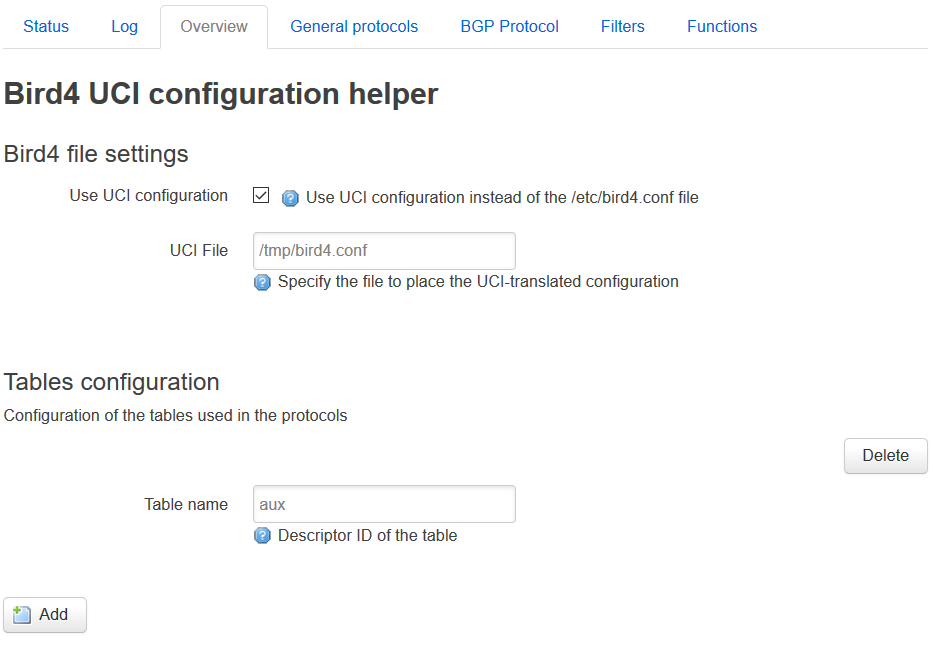
\includegraphics[width=\textwidth]{images/bird0.3/overview}
    \caption{Overview Page}
    \label{fig:overview}
\end{figure}

\textbf{Changes and Improvements:}
This section has not been severely modified. The only big change has been the Log\&Debug settings, because there were some issues using \textit{All} together with other options. By definition, \textit{All} implicitly includes the other options and should be not passed to the configuration.

\subsubsection{General Protocols Page}
The General Protocols Page shows the configuration of some of the supportive protocols described in section \ref{sub:sub:supproto}.

\begin{itemize}
    \item Kernel Protocol (1 mandatory as base Routing Table talking to the OS. Any extra kernel protocol is optional)
    \item Device Protocol: optional
    \item Pipe Protocol: optional
    \item Direct Protocol: optional
    \item Static Protocol: optional
    \item Routes: Routes are just the representation of entries in a Static Protocol. These are optional and tied to a single Static Protocol.
\end{itemize}

\begin{figure}[H]
    \centering
    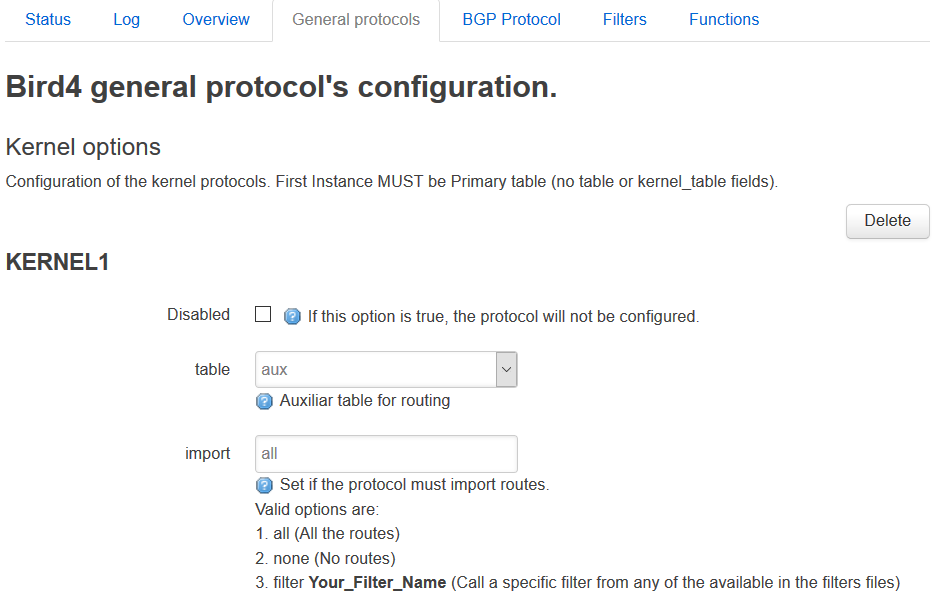
\includegraphics[width=\textwidth]{images/bird0.3/general}
    \caption{General Protocols Page}
    \label{fig:generalp}
\end{figure}

\textbf{Changes and Improvements:}
Main change in this page has been the recovery of both PIPE and Direct Protocols, disabled during the original Project because they were not relevant (there was no coexistence of protocols in Bird). 
These two protocols are now required as they allow to communicate routing tables (PIPE) and to mark the routes as device ones on specific \textit{local} interfaces (DEVICE) to feed the kernel table.

\subsubsection{BGP Protocol Page}
The BGP Protocol Page is the most important for this project as it allows us to configure the main protocol used in Guifi.net. Together with OSPF, BGP is the most complex protocol to configure (and translate) on Bird. With a big number of different \textit{options} as well as another big number of \textit{attributes} to configure, the automation of this protocol has been the main goal of this Package.

\begin{itemize}
    \item Kernel Protocol (1 mandatory as base Routing Table talking to the OS. Any extra kernel protocol is optional)
    \item BGP Templates: allow to set a number of common options repeated among a number of  different BGP Sessions. Their use simplifies configuration's maintainability as well as improves readability of the file. Templates are optional and you can configure as many as required.
    \item BGP Instances: Instances are the definition of each BGP session to be created. They can feed from Templates or set all the options manually. Instance options will always prevail over template ones. Instances are optional and you can configure as many as required.
\end{itemize}

\begin{figure}[H]
    \centering
    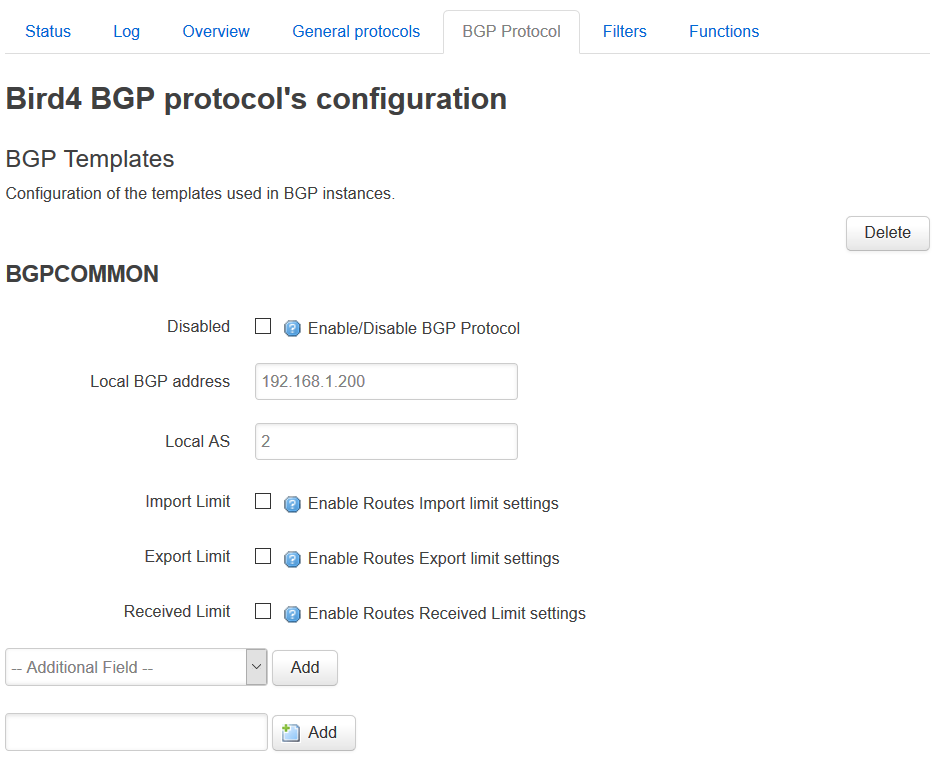
\includegraphics[width=\textwidth]{images/bird0.3/bgp}
    \caption{BGP Protocol Page}
    \label{fig:bgpp}
\end{figure}

\textbf{Changes and Improvements:}

\subsubsection{Filters \& Functions Page}

\begin{figure}[H]
    \centering
    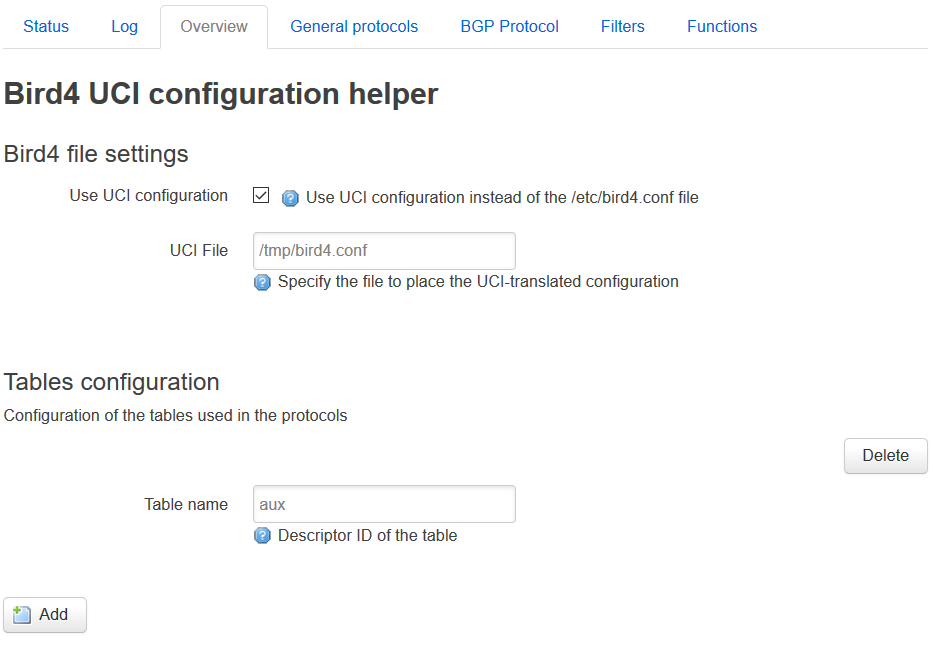
\includegraphics[width=\textwidth]{images/bird0.3/overview}
    \caption{Overview Page}
    \label{fig:overview}
\end{figure}

\subsection{Align documentation and upgrade to Markdown}
%%TBD


